\section{Lo spazio delle fasi}
L'elemento di matrice che abbiamo trovato dipende, oltre che dalle energie, anche dall'angolo fra il neutrino e l'elettrone
$$
\overline{|\mathfrak{M}_F|^2} = 16m_N^2 E_e E_\nu G^2 \left[ C_S^2 (1 - \boldsymbol{\beta}_e \cdot \boldsymbol{\beta}_\nu) + C_V^2 (1 + \boldsymbol{\beta}_e \cdot \boldsymbol{\beta}_\nu) + 2C_S C_V \frac{m_e}{E_e} \right]
$$
Vedremo che la distribuzione di $\theta_{e\nu}$ contiene importanti informazioni. è pertanto necessario sviluppare lo spazio delle fasi senza integrare sugli angoli. Riprendiamo pertanto il calcolo a partire dall'integrazione del momento del protone in poi:
$$
d\Phi = \frac{(2\pi)^4}{(2\pi)^9} \frac{k^2 dk d\Omega_e}{2E_e} \frac{k'^2 dk' d\Omega_\nu}{2E_\nu} \frac{1}{2E_p} \delta(m_n - E_e - E_\nu - \sqrt{\mathbf{k}^2 + \mathbf{k}'^2 + 2kk' \cos\theta_{e\nu} + m_p^2})
$$
Adesso vogliamo integrare sull'energia del neutrino e poniamo $x=E_\nu=|\mathbf{k}'|$
$$
f(x) = m_n - E_e - x - \sqrt{\mathbf{k}^2 + x^2 + 2kx \cos\theta_{e\nu} + m_p^2} = E_p \approx m_p
$$
Trascurando l'energia cinetica del protone
$$
f(x) \approx m_n - m_p - E_e - x = x_0 - x \qquad x_0 \approx m_n - m_p - E_e \qquad |f'(x_0)| = 1 \qquad \delta(f(x)) = \delta(x_0 - x)
$$
Con questa approssimazione abbiamo (ricordiamo $|k'|=E_\nu$ e $p_e$$\equiv|\mathbf{k}|$)
$$
d\Phi = \frac{(2\pi)^4}{(2\pi)^9} \frac{p_e^2 dp_e d\Omega_e}{2E_e} \frac{E_\nu^2 dE_\nu d\Omega_\nu}{2E_\nu} \frac{1}{2E_p} \delta(E_\nu - \overline{E}_\nu)\qquad \overline{E}_\nu = m_n - m_p - E_e \qquad m_n - m_p = \Delta m
$$ 
Possiamo a questo punto integrare su $E_\nu$
$$
d\Phi = \frac{1}{(2\pi)^5} \frac{p_e^2 dp_e d\Omega_e}{8E_e E_p} \overline{E}_\nu d\Omega_\nu
$$
Inoltre utilizziamo la consueta relazione
$$
p_e^2 = E_e^2 - m_e^2 \to p_e dp_e = E_e dE_e
$$
Ancora una volta trascuriamo l'energia cinetica del protone $E_p\approx m_p \approx m_N$
$$
d\Phi = \frac{1}{(2\pi)^5} \frac{E_\nu p_e}{8m_N} dE_e d\Omega_e d\Omega_\nu
$$
Per semplicità abbiamo sostituito $\overline{E}_\nu=E_\nu=m_n-m_p-E_e$. A questo punto abbiamo tutti gli ingredienti per il calcolo della larghezza di decadimento.
\section{La larghezza di decadimento}
In definitiva abbiamo per la larghezza delle transizioni di fermi
$$
d\Gamma_F = \frac{1}{2m_n} |\mathfrak{M}_F|^2 d\Phi
$$
$$
d\Gamma_F = \frac{1}{2m_N} 16m_N^2 E_e E_\nu G^2 \left[ C_S^2 (1 - \boldsymbol{\beta}_e \cdot \boldsymbol{\beta}_\nu) + C_V^2 (1 + \boldsymbol{\beta}_e \cdot \boldsymbol{\beta}_\nu) + 2C_S C_V \frac{m_e}{E_e} \right] \frac{1}{(2\pi)^5} \frac{E_\nu p_e}{8m_N} dE_e d\Omega_e d\Omega_\nu
$$
$$
d\Gamma_F = G^2 \frac{(C_S^2 + C_V^2)}{(2\pi)^5} p_e E_e E_\nu^2 \left[ 1 + a_F \boldsymbol{\beta}_e \cdot \boldsymbol{\beta}_\nu + \kappa_F \frac{m_e}{E_e} \right] dE_e d\Omega_e d\Omega_\nu
$$
Dove
$$
E_\nu = \Delta m - E_e \qquad a_F = \frac{C_V^2 - C_S^2}{C_S^2 + C_V^2} \qquad \kappa_F = \frac{2C_S C_V}{C_S^2 + C_V^2}
$$
Analogamente per la larghezza delle transizioni di Gamov-Teller
$$
d\Gamma_{GT} = G^2 \frac{3(C_A^2 + C_T^2)}{(2\pi)^5} p_e E_e E_\nu^2 \left[ 1 + a_{GT} \boldsymbol{\beta}_e \cdot \boldsymbol{\beta}_\nu - \kappa_{GT} \frac{m_e}{E_e} \right] dE_e d\Omega_e d\Omega_\nu
$$
Dove
$$
a_{GT} = -\frac{1}{3} \frac{C_A^2 - 4C_T^2}{C_A^2 + 4C_T^2} \qquad \kappa_{GT} = 4 \frac{2C_A C_T}{C_A^2 + C_T^2}
$$
\section{La distribuzione dell'energia}
-Con un po' di manipolazioni dell'elemento di matrice siamo arrivati alle due forme molto simili della larghezza di decadimento per i processi di Fermi o di Gamow-Teller parametrizzati da delle quantità sconosciute che sono la $a_F$ e la $k_F$ per le transizioni di Fermi e $a_GT$ e $k_GT$ per quelle di Gamow-Teller. Quello che faremo è andare a vedere quali sono le conseguenze fenomenologiche di questi parametri che vogliamo misurare o meglio gli effetti che sperimentalmente bisogna misurare per vedere che valore hanno questi parametri.

Importante è il prodotto scalare tra i due beta. Siamo interessati solo alla distribuzione dell'energia. Quando integriamo su tutto l'angolo solido questo termine scompare e quindi il termine di energia è sensibile solo al termine k e non al termine a. Fissiamo la direzione dell'elettrone e quindi possiamo integrare rispetto ai due angoli solidi.

Si nota come la curva effettivamente cambia in funzione che questo termine di interferenza sia uguale o diverso da 1. Che sperimento riesce a capire di quale curva si tratta? k=0 è una informazione importantissima! Visto che o $C_S$ o $C_V$ deve essere uguale a zero. Quindi quando noi diciamo che le transizioni di Fermi e quindi quelle che non permettono la variazione dello spin devono essere o scalari o vettoriali questo k=0 ci dice che deve essere per forza O scalari O vettoriali Ma non tutti e due quindi di quei termini ce ne solo uno e questo discorso vale anche per Gamow-Teller. Una misura "semplice" fatta con una precisione comunque considerevole porta a delle conclusioni importantissime! Un'altra misura poi ci dirà quale delle due rimane
-
Cominciamo con lo studio della distribuzione dell'energia dell'elettrone. Ricordiamo che l'elemento di matrice dipende da termini che contengono
$$
\boldsymbol{\beta}_e \cdot \boldsymbol{\beta}_\nu = \beta_e \beta_\nu \cos\theta_{e\nu} = \beta_e \cos\theta_{e\nu}
$$
Lo spazio delle fasi dipende dalle direzioni $d\Omega_e$ e $d\Omega_\nu$ dei momenti dell'elettrone e del neutrino. Misuriamo gli angoli rispetto alla direzione dell'elettrone (possiamo quindi integrare su $d\Omega_e\to4\pi$). L'integrale sull'angolo solido del neutrino di questi termini dà contributo nullo
$$
\int_{-1}^{+1} \cos\theta_\nu d\cos\theta_\nu = 0
$$
Per i termini dell'elemento di matrice che non dipendono dagli angoli degli integrali sui due angoli solidi equivalgono a moltiplicare per $16\pi^2$. In definitiva, per una transizione di Fermi
$$
\frac{d\Gamma_F}{dE_e} = 4G^2 \frac{(C_S^2 + C_V^2)}{(2\pi)^3} p_e E_e (\Delta m - E_e)^2 \left[ 1 + \kappa_F \frac{m_e}{E_e} \right]
$$
Ricordiamo che abbiamo usato l'approssimazione $E_\nu\approx\delta m-E_e$. Le prime informazioni sulla struttura della interazione debole nel decadimento $\beta$ sono state ottenute studiando lo spettro della energia dell'equazione precedente. Il termine con coefficiente $\kappa_F$ è un termine di interferenza è noto come Termine di interferenza di Fierz (N.B.: il valore minimo di $E_e$ è $m_e$). Dallo studio della forma dello spettro si può verificare l'esistenza o meno del termine di interferenza. I risultati sperimentali mostrano che questo termine è assente ($\kappa=0$) sia per le transizioni di Fermi che per le transizioni di Gamov-Teller.
\begin{figure}[h!]
	\centering
	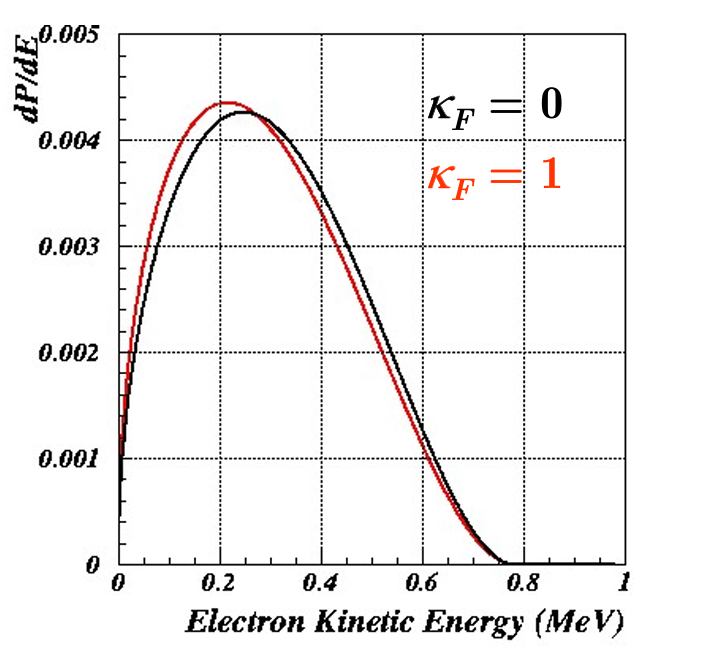
\includegraphics[width=0.8\textwidth]{Lezioni/Lezione 13/op.png}
	\label{fig:op}
\end{figure}
L'assenza del termine di interferenza di Fierz ha delle conseguenze importanti. Ricordiamo la forma dei coefficienti dei termini di interferenza
$$
\kappa_F=\frac{2C_SC_V}{C_S^2+C_V^2} \qquad \kappa_{GT}=\frac{2C_AC_T}{C_A^2+C_T^2}
$$
La condizione $\kappa_{F,GT}=0$ implica che solo uno dei due accoppiamenti può essere presente
$$
C_SC_V=0\qquad C_AC_T=0
$$
Pertanto dei $4$ possibili tipi di interazione solo $2$ dovevano essere presenti con le seguenti possibilità:
\begin{itemize}
	\item Scalare - Assiale
	\item Scalale - Tensoriale
	\item Vettoriale - Assiale
	\item Vettoriale - Tensoriale
\end{itemize}
Da un punto di vista sperimentale è interessante studiare i requisiti di risoluzione e di precisione statistica per stabilire l'assenza o meno dei termini di interferenza. Ovviamente, per misurare lo spettro di energia, abbiamo bisogno di un rivelatore che misuri l'energia di ogni singolo elettrone che lo attraversa. Una prima caratteristica importante è la necessità di assorbire tutta l'energia. Ma la caratteristica più importante è sicuramente la risoluzione [vedi slide 347-349].
\subsection*{Effetto della Risoluzione Strumentale sullo Spettro di Energia: La Convoluzione}

Nello studio sperimentale del decadimento $\beta$, l'osservabile fisica fondamentale è lo spettro continuo dell'energia dell'elettrone. Tuttavia, nessun rivelatore è ideale: ogni misura è affetta da un errore intrinseco (rumore elettronico) che "spalma" il valore dell'energia vera secondo una distribuzione statistica, tipicamente gaussiana. 

\subsubsection*{Dal caso discreto al limite continuo}
Supponiamo inizialmente che la sorgente emetta elettroni a energie discrete $E_i$, ciascuna con un "peso" o probabilità di emissione $f_i$. A causa della risoluzione finita del rivelatore (caratterizzata da una deviazione standard $\sigma$), l'energia misurata $E$ non corrisponderà esattamente a $E_i$, ma sarà distribuita secondo una gaussiana $G(E - E_i)$ centrata in $E_i$.

La probabilità totale $P(E)$ di leggere sul rivelatore un'energia $E$ è data dalla somma dei contributi pesati delle singole gaussiane:
\begin{equation}
	P(E) \approx \sum_i f_i \cdot G(E - E_i) \Delta E
\end{equation}

Nel caso reale del decadimento $\beta$, lo spettro non è discreto ma continuo. La teoria ci fornisce una funzione di distribuzione teorica dell'energia $f(x)$, dove $x$ rappresenta l'energia vera (cinematica) della particella. Effettuando il passaggio al limite per intervalli di energia infinitesimi ($\Delta E \to dx$), la sommatoria si trasforma rigorosamente in un integrale:
\begin{equation}
	P(E) = \int f(x) G(E - x) dx
\end{equation}
Questa operazione matematica rappresenta esattamente la \textbf{convoluzione} dello spettro teorico $f(x)$ con la funzione di risoluzione del rivelatore $G$.

\subsubsection*{Significato Fenomenologico e Termine di Fierz}
Questo passaggio matematico è di cruciale importanza fenomenologica. Il nostro obiettivo teorico è studiare la forma esatta di $f(x)$, poiché essa dipende dal \textbf{termine di interferenza di Fierz} ($k_F$). Il valore di $k_F$ è fondamentale: misurare $k_F = 0$ implica che nella Lagrangiana di interazione debole possono coesistere o accoppiamenti (Scalare e Tensoriale) o (Vettoriale e Assiale), ma non forme incrociate.

Il problema sperimentale risiede nel fatto che \textit{non è possibile misurare direttamente $f(x)$}. Il rivelatore restituisce sempre e solo lo spettro "smearingato" $P(E)$. 

Di conseguenza, per estrarre il parametro $k_F$, la procedura corretta consiste nel:
\begin{enumerate}
	\item Calcolare teoricamente $f(x)$ (dipendente da $k_F$) tramite la Regola d'Oro di Fermi e il calcolo delle tracce di Dirac.
	\item Effettuare analiticamente o numericamente la \textbf{convoluzione} di $f(x)$ con la gaussiana della risoluzione strumentale $G$.
	\item Eseguire un fit della funzione risultante $P(E)$ sui dati sperimentali.
\end{enumerate}
Solo tramite questo confronto rigoroso tra teoria (convoluta) ed esperimento è stato possibile dimostrare l'assenza del termine di Fierz ($k_F = 0$) e orientare la formulazione della Teoria V-A.

\section{Correlazione angolare e - nu}
-voglio andare a vedere cosa succede alla distribuzione della larghezza di decadimento rispetto all'energia e all'angolo del neutrino se metto CS=0 o CV=0

Questo vuol dire che se l'accoppiamento è di tipo vettoriale e quindi lo scalare non c'è allora l'elettrone e il neutrino saranno tendenzialmente collineari e quindi emessi paralleli. Viceversa se va a zero il CV il coefficiente è -1 e quindi acrei un massimo se vengono emessi back to back. ovvimente i vari angoli sono permessi ma ma statisticamente sono favoritideterminati ngoli. fenomenologicamente possiao andare a studiare se c'è una o c'è l'altra. Possiamo fare lo stesso discorso per la larghezza di Gamow-Teller.

ESPERIMENTO DI ALLEN
una prima caratteristica non banale (abbiamo visto che le energie in gioco sono molto basse quindi se ho un nucleo che rincula questo perde subito tutta la sua energia e non vedrò le direzioni) questo si può ovviare lavorando nel vuoto o bassissima densità in modo tale che il nucleo dopo l'emissione potesse viaggiare un pochino. Oggettino piccolo ma difficile da fare. Helio-6 è da fare in un luogo vicino a dove può essere prodotto (ciclotrone!).
-
Richiamiamo le espressioni delle larghezze di Fermi e Gamov-Teller. Includiamo il risultato sperimentale $C_S$ $C_V=C_A$ $C_T=0$ ($\kappa_F=\kappa_{GT}=0$)
$$
d\Gamma_F = G^2 \frac{(C_S^2 + C_V^2)}{(2\pi)^5} p_e E_e E_\nu^2 [1 + a_F \boldsymbol{\beta}_e \cdot \boldsymbol{\beta}_\nu ] dE_e d\Omega_e d\Omega_\nu
$$
$$
d\Gamma_{GT} = G^2 \frac{3(C_A^2 + C_T^2)}{(2\pi)^5} p_e E_e E_\nu^2 [1 + a_{GT} \boldsymbol{\beta}_e \cdot \boldsymbol{\beta}_\nu ] dE_e d\Omega_e d\Omega_\nu
$$
Cominciamo con l'elemento di matrice delle transizioni di Fermi, poichè |$\beta_\nu=1$|, esprimendo il prodotto scalare in funzione dell'angolo fra elettrone e il neutrino, integrando su $d\Omega_e$, otteniamo ($A$ costante)
$$
\frac{d\Gamma_F}{dE_e d\Omega_\nu} = A [1 + a_F \beta_e \cos(\theta_{e\nu})] \quad a_F = \frac{C_V^2 - C_S^2}{C_S^2 + C_V^2}
$$
Pertanto se $a_F>0$ ($C_S=0$) la distribuzione ha un massimo se elettrone e neutrino tendono a essere collineari $\to$ $\cos{\theta_{e\nu}}=1$. Se invece $a_f<0$ ($C_V=0$) la distribuzione ha un massimo se elettrone e neutrino tendono ad andare in direzione opposta $\to$ $\cos{\theta_{e\nu}}=-1$. Analogamente la larghezza di Gamov-Teller
$$
\overline{|\mathfrak{M}_{GT}|^2} = 16m_N^2 E_e E_\nu 3 G^2 (C_A^2 + 4C_T^2) [1 + a_{GT} \boldsymbol{\beta}_e \cdot \boldsymbol{\beta}_\nu]
$$
Con $a_{GT}>0\to$ Tensoriale, conduce alla distribuzione angolare
$$
\frac{d\Gamma_{GT}}{dE_e d\Omega_\nu} = B [1 + a_{GT} \beta_e \cos(\theta_{e\nu})] \quad a_{GT} = -\frac{1}{3} \frac{C_A^2 - 4C_T^2}{C_A^2 + 4C_T^2}
$$
con $a_{GT}<0\to$ Assiale. Quando si ha il massimo della distribuzione? Ovviamente il neutrino non può essere rivelato ma si possono però misurare l'energia e/o la direzione del nucleo che rincula e utilizzare la conservazione della quantità di moto. Ci sono 5 variabili ($P_e$., $P_\nu$, $P_p$, $\theta_e$, $\theta_p$) e 3 equazioni. In un esperimento ideale: si determinano due grandezze misurabili, si ricava $\theta_{e\nu}$, si costruisce la distribuzione di $\cos{\theta_{e\nu}}$ e si misura $a_{GT}$ (o $a_F$)
$$
\begin{cases}
	P_\nu = P_e \cos\theta_e + P_p \cos\theta_p \\
	P_e \sin\theta_e = P_p \sin\theta_p \\
	m_n - m_p = P_\nu + T_p + E_e
\end{cases}
$$
\subsection{Esperimento di Allen et al}
\begin{figure}[h!]
	\centering
	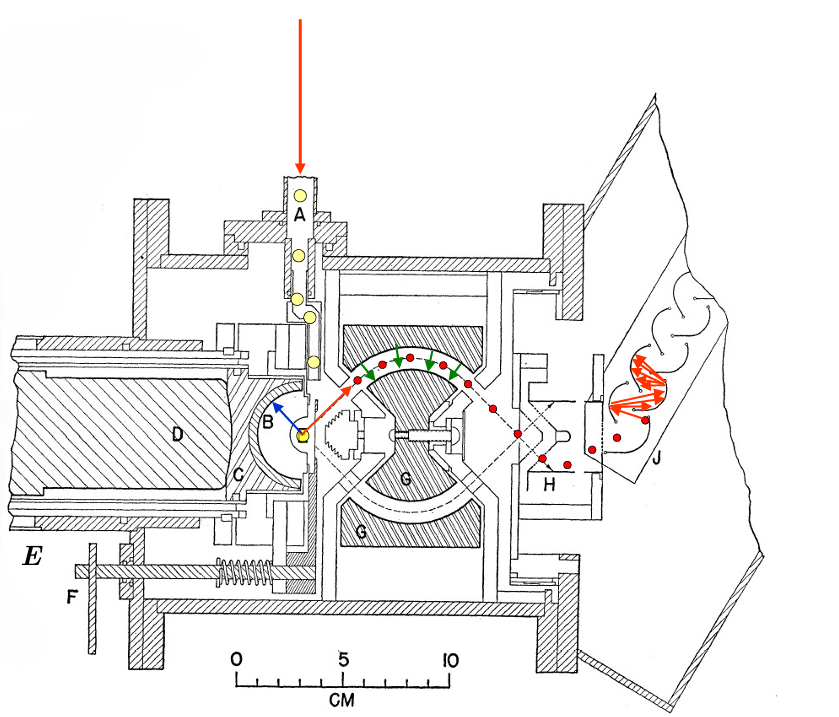
\includegraphics[width=0.7\textwidth]{Lezioni/Lezione 13/tr.png}
	\label{fig:tr}
\end{figure}
Per poter misurare l'energia di rinculo si deve studiare il decadimento nel vuoto. Il gas radioattivo, prodotto con un ciclotrone viene immesso dal condotto. I nuclei radioattivi diffondono nell'apparato. I decadimento utili sono quelli che avvengono nella zona $E$. Gli elettroni sono rivelati in $B$ e tramite un campo elettrico $E$ i nuclei (ioni) vengono selezionati in energia con G e vengono rivelati in H-J. Quindi si misura la distribuzione dell'energia cinetica del nucleo. Ci sono solo due direzione del rinculo che entrano nello spettrometro e gli eventi selezionati sono quelli in cui l'angolo fra nucleo ed elettrone varia da $\theta_{min}$ a $\theta_{max}$. Altri conti nella slide 354. La distribuzione di energie del nucleo non si può ottenere analiticamente. Occorre un calcolo numerico o una simulazione Montecarlo.
\subsection{Riepilogo}
Conseguenza dello studio dello spettro dell'energia dell'elettrone: nelle transizioni di Fermi e Gamov-Teller sono assenti i termini di interferenza. 
\begin{itemize}
	\item Dato che $C_S$ $C_V=0$ nelle transizioni di Fermi è attiva solo o la componente Scalare o la componente Vettoriale.
	\item Dato che $C_T$ $C_A=0$ nelle transizioni di Gamov-Teller è attiva solo o la componente Tensoriale o la componente Assiale
\end{itemize}
Dalle informazioni precedenti e dallo studio dell'energia di rinculo del nucleo si ottengono informazioni sulla correlazione angolare $\beta_e-\beta_\nu$.
$$
\text{Interazione di Fermi } \quad a_F=\frac{C_V^2-C_S^2}{C_V^2+C_S^2}=1 \qquad C_S=0 \quad C_V\not=0
$$
$$
\text{Interazione di Gamov-Teller } \quad a_{GT}=-\frac{1}{3}\frac{C_A^2-C_T^2}{C_A^2+C_T^2}=-\frac{1}{3} \qquad C_T=0 \quad C_A\not=0
$$
Pertanto l'Hamiltoniana del decadimento $\beta$ contiene solo i seguenti termini:
$$
\text{Vettoriale } \quad \gamma^\mu \qquad \qquad \text{Vettoriale assiale } \quad \gamma^5\gamma^\mu
$$
C'è un'altra cosa da sottolineare: noi abbiamo visto che siccome è difficile misurare gli eventi singolarmente risulta migliore! Qui c'è un dato importante dal punto di vista della fisica sperimentale. Al crescere dell'angolo su cui integriamo il metodo perde sensibilità. Cioè quando io vado a fare il risultato di un fit e vedo che errore ho su a l'errore diventa sempre più grande a parità di statistica. Dovrei aumentare di più la statistica quindi. Questa cosa c'è sempre. Man mano che integriamo perdiamo informazione e il caso limite migliore è quando prendiamo un evento singolo per volta. 
\section{La vita media}
Infine possiamo calcolare la vita media. Assumendo assenti i termini di interferenza ($\kappa=0$) abbiamo (Fermi)
$$
d\Gamma_F = 4G^2 \frac{(C_S^2 + C_V^2)}{(2\pi)^3} p_e E_e E_\nu^2 dE_e
$$
Abbiamo inoltre visto che è presente solo il termine vettoriale ($C_S=0$) perché misurato dall'esperimento di Allen
$$
d\Gamma_F = 4G^2 \frac{C_V^2}{(2\pi)^3} p_e E_e E_\nu^2 dE_e
$$
Analogamente nelle transizioni di Gamov-Teller è presente solo il termine assiale ($C_T=0$) e pertanto risulta
$$
d\Gamma_{GT} = 4G^2 \frac{3C_A^2}{(2\pi)^3} p_e E_e E_\nu^2 dE_e
$$
In un decadimento in cui sono presenti entrambi i termini abbiamo
$$
d\Gamma = \frac{4}{(2\pi)^3} G^2 (C_V^2 + 3C_A^2) p_e E_e E_\nu^2 dE_e
$$
Conviene riscrivere l'ultima equazione come
$$
d\Gamma = \frac{4}{(2\pi)^3} G^2 C_V^2 \left( 1 + 3 \frac{C_A^2}{C_V^2} \right) p_e E_e E_\nu^2 dE_e
$$
La larghezza totale è data pertanto dall'integrale
$$
\Gamma = \frac{4}{(2\pi)^3} G^2 C_V^2 \left( 1 + 3 \frac{C_A^2}{C_V^2} \right) \int_{m_e}^{m_e+\Delta m} |\mathbf{k}| E_e E_\nu^2 dE_e \qquad \left[ \int_{m_e}^{m_e+\Delta m} \right] = M^5
$$
Notiamo le dimensioni dell'integrale: in realtà per misure di precisione occorre tenere conto di effetti che per semplicità finora abbiamo trascurato. Elemento di matrice nucleare e effetti del campo coulombiano. Nell'elemento di matrice nucleare abbiamo assunto (per semplificare)
$$
|\langle \boldsymbol{\sigma} \rangle|^2 = |\langle \sigma_x \rangle|^2 + |\langle \sigma_y \rangle|^2 + |\langle \sigma_z \rangle|^2 = 3 \qquad |\langle 1 \rangle|^2 = 1
$$
Per tenere conto degli elementi di matrice nucleare si definisce (e si calcola)
$$
\xi = |\langle 1 \rangle|^2 + \frac{C_A^2}{C_V^2} |\langle \boldsymbol{\sigma} \rangle|^2 \qquad G_\beta = G C_V\qquad \Gamma = \frac{4}{(2\pi)^3} G_\beta^2 \xi \int_{m_e}^{m_e+\Delta m} |\mathbf{k}| E_e E_\nu^2 dE_e
$$
Ovviamente con la sola misura di $\Gamma$ non è possibile separare $G$ e $C_V$. Qui c'è un capitolo di fisica molto interessante che approfondiremo nelle prossime lezioni. Per ora questo $GC_V$ lo chiamiamo appunto $G_\beta$ che vuol dire la costante di Fermi determinata dal decadimento beta nucleare. Questo perché $C_V$ è sostanzialmente $1$ ma non è proprio $1$ ma poco meno. Quindi è praticamente la costante. Questo valore cambia se vado a studiare il decadimento del muone mediato dall'interazione debole. Facendo gli stessi esperimenti con i muoni troveremo una costante di Fermi fatta in questo modo che è leggermente diversa perché nel caso dei muoni questo $C_V$ è esattamente uguale a $1$. Queste costanti quindi sono leggermente differenti. Questa differenza deriva dal fatto che protone e neutrone non sono puntiformi (che è quello che vorrebbe l'equazione di Dirac ma è invece un sistema composito di di particelle puntiformi). Ci torneremo. Ritorneremo in seguito sul rapporto $C_A/C_V$. Per tenere conto dell'effetto del campo coulombiano che modifica le funzioni d'onda dell'elettrone (abbiamo usato le funzioni d'onda di particelle libere) si introduce la funzione di Fermi $F(Z,E_e)$ che moltiplica l'integranda e si definisce:
$$
f = \int_{m_e}^{m_e+\Delta m} F(Z, E_e) p_e E_e (\Delta m - E_e)^2 dE_e
$$
Abbiamo in definitiva (dipende dal quanto è intenso il campo coulombiano Z e dall'energia dell'elettrone)
$$
\Gamma = \frac{1}{\tau} = \frac{G_\beta^2}{2\pi^3} \xi f
$$
Sperimentalmente si studia
$$
f\tau = \frac{2\pi^3}{G_\beta^2 \xi}\to ft_{1/2} = \frac{2\pi^3 \ln 2}{G_\beta^2 \xi}
$$
Misurando la vita media di un decadimento di un nucleo e calcolato il valore di $\xi$ per quel nucleo si ottiene $G_\beta$. Questo valore misurato e mediato su tanti decadimenti è
$$
G_\beta = 1.13578 \pm 0.00027 \times 10^{-5} \, \text{GeV}^{-2}
$$
\section{Il gruppo di Lorentz}
La richiesta che le leggi fisiche siano le stesse in tutti i sistemi inerziali implica che le grandezze fisiche abbiano ben precise leggi di trasformazione rispetto alle trasformazioni di Lorentz. In particolare i $4-$vettori. Infatti questi hanno un modulo invariante per trasformazioni $m^2 = g_{\mu\nu} p^\mu p^\nu$. Matematicamente le trasformazioni di Lorentz possono essere definite come le trasformazioni che lasciano invariata la forma quadratica $g_{\mu\nu}x^\mu y^\nu$. Abbiamo visto che la condizione necessaria e sufficiente perchè ciò accada è che la matrice $\Lambda$ che rappresenta la trasformazione abbia la proprietà
$$
g_{\mu\nu} \Lambda^\mu_\alpha \Lambda^\nu_\beta = g_{\alpha\beta} \qquad \Lambda^T G \Lambda = G
$$
Che può essere scritta in maniera equivalente come $\Lambda_\mu^\alpha \Lambda^\mu_\beta = \delta^\alpha_\beta$. Questo significa che la matrice inversa $\Lambda^{-1}$ è data da $(\Lambda^{-1})^\nu_\mu = \Lambda_\mu^\nu$. Si tratta di una trasposizione e di cambi di segno (elementi $\Lambda_0^i$ \quad e $\Lambda_i^0$). Le matrici $\Lambda$ che soddisfano le condizioni enunciate formano un gruppo: Il Gruppo di Lorentz. Questo gruppo ha le solite proprietà: chiusura, associatività, identità, inversa e tante altre visibili nella slide 361. Il gruppo definito in modo astratto contiene molto di più che delle semplici trasformazioni di Lorentz (boost) ovviamente anche le rotazioni e contiene gli operatori di inversione temporale $\mathbb{T}$ e inversione spaziale $\mathbb{P}$
$$
\mathbb{T}^\mu_{\,\,\,\nu} = \begin{pmatrix}
	-1 & 0 & 0 & 0 \\
	0 & 1 & 0 & 0 \\
	0 & 0 & 1 & 0 \\
	0 & 0 & 0 & 1
\end{pmatrix} \qquad \mathbb{P}^\mu_{\,\,\,\nu} = \begin{pmatrix}
1 & 0 & 0 & 0 \\
0 & -1 & 0 & 0 \\
0 & 0 & -1 & 0 \\
0 & 0 & 0 & -1
\end{pmatrix}
$$
Questi operatori sono di natura diversa rispetto alle trasformazioni di Lorentz fin qui studiate. Non si possono costruire a partire dall'identità come somma di operazioni infinitesime e non possono essere "connesse" con continuità all'identità. Sono trasformazioni discrete. Una qualsiasi trasformazione del gruppo di Lorentz può essere costruita combinando: boost, rotazioni, inversioni $\mathbb{T}$ e inversione $\mathbb{P}$.
\subsection{Classificazione del gruppo di Lorentz}
Esaminiamo in maggiore dettaglio la struttura del gruppo di Lorentz. Una prima classificazione fatta sulla base del segno del determinante. Abbiamo visto che $(\text{det}[\Lambda])^2=1$ e quindi $\text{det}[\Lambda]=\pm1$. Si definiscono quindi i due seguenti tipi di trasformazioni:
\begin{itemize}
	\item Se $\text{det}[\Lambda]=+1$ allora si dice Trasformazioni di Lorentz proprie 
	\item Se $\text{det}[\Lambda]=-1$ allora si dice Trasformazioni di Lorentz improprie 
\end{itemize}
Notiamo che il prodotto di due trasformazioni proprie è ancora una trasformazione propria ma questa proprietà non vale per le trasformazioni improprie. La seconda classificazione viene fatta sulla base del segno dell'elemento $\Lambda^0_{\,\,\,0}$. Specializzando la relazione $\Lambda^TG\Lambda=G$ all'indice $00$ di G
$$
g_{\mu\nu} \Lambda^\mu_\alpha \Lambda^\nu_\beta = g_{\alpha\beta} \quad \Longrightarrow \quad g_{\mu\nu} \Lambda^\mu_0 \Lambda^\nu_0 = g_{00} = 1 \qquad 1 = \Lambda^0_0 \Lambda^0_0 - \sum_i \Lambda^i_0 \Lambda^i_0
$$
$$
\Lambda^0_0 \Lambda^0_0 = 1 + \sum_i (\Lambda^i_0)^2 \qquad (\Lambda^0_0)^2 \ge 1 \qquad \Lambda^0_0 \ge +1 \qquad \Lambda^0_0 \le -1
$$
Si definiscono i due seguenti tipi di trasformazioni:
\begin{itemize}
	\item Se $\Lambda_{\,\,\,0}^0\ge+1$ sono Trasformazioni di Lorentz ortocrone
	\item Se $\Lambda_{\,\,\,0}^0\le+1$ sono Trasformazioni di Lorentz non-ortocrone
\end{itemize}
Le trasformazioni del gruppo di Lorentz sono pertanto classificati per il segno del determinante e per il segno del termine $\Lambda_{\,\,\,0}^0$. Nella tabella $\Lambda^{(po)}$ si intende trasformazione propria e ortocrona.


\begin{tabular}{|c|c|c|}
	\hline
	& $\mathbf{\Lambda^0_0 \ge +1}$ & $\mathbf{\Lambda^0_0 \le -1}$ \\
	& \textbf{ortocrona} & \textbf{non-ortocrona} \\
	\hline
	$\mathbf{\det[\Lambda] = +1}$ & & \\
	\textbf{propria} & $\Lambda^{(\text{po})}$ & $T P \Lambda^{(\text{po})}$ \\
	\hline
	$\mathbf{\det[\Lambda] = -1}$ & & \\
	\textbf{impropria} & $P \Lambda^{(\text{po})}$ & $T \Lambda^{(\text{po})}$ \\
	\hline
\end{tabular}


Le trasformazioni delle altre classi si ottengono combinando $\Lambda^{(po)}$, $\mathbb{T}$ e $\mathbb{P}$, è facile verificare che:
\begin{itemize}
	\item $I$ è propria e ortocrona
	\item $\mathbb{P}$ è impropria e ortocrona
	\item $\mathbb{T}$ è impropria e non ortocrona
	\item Le trasformazioni $\Lambda^{(po)}$ sono un sottogruppi
	\item Le trasformazioni proprie sono un sottogruppo
	\item Le trasformazioni proprie ortocrone sono un sottogruppo
	\item L'insieme delle trasformazioni proprie ortocrone e delle trasformazioni improprie e non-ortocrone sono un sottogruppo
\end{itemize}
NB: i boost non sono un sottogruppo infatti due boost in direzioni diverse sono equivalenti ad un boost più una rotazione.
\section{Inversione degli spinori}
In precedenza abbiamo visto come costruire le trasformazioni di Lorentz per uno spinore. Erano trasformazioni associate a trasformazioni proprie e ortocrone costruite come somma di trasformazioni infinitesime a partire dall'identità. Ricordiamo la condizione di invarianza della equazione di Dirac: la trasformazione $S(\Lambda)$ e le matrici $\gamma$ avevano la seguente proprietà
$$
S^{-1}(\Lambda)\gamma^\mu S(\Lambda) = \Lambda^\mu_{\,\,\,\nu} \gamma^\nu
$$
Vogliamo adesso trovare la trasformazione $S_p\equiv S(\mathbb{P})$ che corrisponde all'inversione spaziale $\mathbb{P}$
$$
\Lambda^\mu_\nu = \mathbb{P}^\mu_\nu = \begin{pmatrix} 1 & 0 & 0 & 0 \\ 0 & -1 & 0 & 0 \\ 0 & 0 & -1 & 0 \\ 0 & 0 & 0 & -1 \end{pmatrix}
$$
Scriviamo adesso per esteso le condizioni sulle matrici $\gamma$ per l'invarianza
$$
S_P^{-1}\gamma^0 S_P = \mathbb{P}^0_\nu \gamma^\nu \qquad S_P^{-1}\gamma^0 S_P = \gamma^0
$$
$$
S_P^{-1}\gamma^i S_P = \mathbb{P}^i_\nu \gamma^\nu \qquad S_P^{-1}\gamma^i S_P = -\gamma^i
$$
un operatore con le proprietà di $S_p$ si trova definendo $S_p=\eta\gamma^0$
$$
(\eta\gamma^0)^{-1}\gamma^0(\eta\gamma^0) = \eta^{-1}\gamma^0\gamma^0\eta\gamma^0 = \gamma^0
$$
$$
(\eta\gamma^0)^{-1}\gamma^i(\eta\gamma^0) = \eta^{-1}\gamma^0\gamma^i\eta\gamma^0 = \gamma^0\gamma^i\gamma^0 = -\gamma^i
$$
Scegliamo $\eta=+1$ ed infine richiediamo
$$
\eta = +1 \qquad \overline{S_P}S_P = I \qquad \overline{\eta\gamma^0}\eta\gamma^0 = \eta^*\eta\gamma^0\gamma^0 = |\eta|^2 I \qquad |\eta|^2 = 1
$$
\subsection{Trasformazione dei covarianti bilineari}
Nel calcolo dell'elemento di matrice dell'interazione di Fermi generalizzata abbiamo trovato le seguenti quantità (bilineari covarianti)
$$
f=\overline{u}\Gamma_Xu
$$
Per ogni matrice $\Gamma$ la quantità $f$ è un numero. Le matrici $\Gamma_X$ possono avere indici. Ad esempio $\gamma^\mu$, nel qual caso anche $f$ ha gli stessi indici $f^\mu=\overline{u}\gamma^uu$. Le matrici $\Gamma_i$ sono combinazioni di matrici $\gamma$ che introducono ben precise proprietà di trasformazione di Lorentz per le quantità $f$
\begin{itemize}
	\item $\Gamma_S = 1$ \hfill \textbf{Scalare} \hfill $f = \overline{u} u$
	\item $\Gamma_V = \gamma^\mu$ \hfill \textbf{Vettore} \hfill $f^\mu = \overline{u} \gamma^\mu u$
	\item $\Gamma_A = \gamma^5 \gamma^\mu$ \hfill \textbf{Vettore Assiale} \hfill $f^\mu = \overline{u} \gamma^5 \gamma^\mu u$
	\item $\Gamma_T = \sigma^{\mu\nu} = i/2 [\gamma^\mu, \gamma^\nu]$ \hfill \textbf{Tensore} \hfill $f^{\mu\nu} = \overline{u} \gamma^\mu \gamma^\nu u$
	\item $\Gamma_P = \gamma^5$ \hfill \textbf{Pseudoscalare} \hfill $f = \overline{u} \gamma^5 u$
\end{itemize}
Verifichiamo adesso le proprietà di trasformazione delle grandezze $f$ per trasformazioni di Lorentz proprie e ortocrone $S(\Lambda)$ e per inversione spaziale $S_P$.
\subsection{Matrice scalare $\Gamma_S = I$}
\begin{itemize}
	\item \textbf{Trasformazione di Lorentz}
	\[
	f' = \overline{u}' \Gamma_S u' = \overline{S u} \Gamma_S S u = \overline{u} \overline{S} S u = \overline{u} u = f
	\]
	Nota: $\overline{S}S = S^{-1}S = I$.
	\item \textbf{Inversione spaziale}
	\[
	f' = \overline{S_P u} \Gamma_S S_P u = \overline{u} \overline{\gamma^0} \gamma^0 u = \overline{u} u = f
	\]
\end{itemize}

\subsection{Matrice vettoriale $\Gamma_V = \gamma^\mu$}
Nota: $S^{-1}(\Lambda)\gamma^\mu S(\Lambda) = {\Lambda^\mu}_\nu \gamma^\nu$.
\begin{itemize}
	\item \textbf{Trasformazione di Lorentz}
	\[
	f'^\mu = \overline{S u} \Gamma_V S u = \overline{u} \overline{S} \gamma^\mu S u = \overline{u} S^{-1} \gamma^\mu S u = \overline{u} {\Lambda^\mu}_\nu \gamma^\nu u = {\Lambda^\mu}_\nu \overline{u} \gamma^\nu u = {\Lambda^\mu}_\nu f^\nu
	\]
	\item \textbf{Inversione spaziale}
	\[
	f'^\mu = \overline{S_P u} \Gamma_V S_P u = \overline{u} \gamma^0 \gamma^\mu \gamma^0 u = 
	\begin{cases} 
		+\overline{u} \gamma^0 u & \mu = 0 \\ 
		-\overline{u} \gamma^i u & \mu = 1,3 
	\end{cases}
	\]
	Questo comportamento definisce un \textbf{Vettore polare}.
\end{itemize}

\subsection{Matrice vettoriale assiale $\Gamma_A = \gamma^5 \gamma^\mu$}
Nota: $\gamma^\mu \gamma^\nu \gamma^5 = \gamma^5 \gamma^\mu \gamma^\nu \rightarrow S \gamma^5 = \gamma^5 S$.
\begin{itemize}
	\item \textbf{Trasformazione di Lorentz}
	\[
	f'^\mu = \overline{S u} \Gamma_A S u = \overline{u} \overline{S} \gamma^5 \gamma^\mu S u = \overline{u} \gamma^5 S^{-1} \gamma^\mu S u = {\Lambda^\mu}_\nu \overline{u} \gamma^5 \gamma^\nu u = {\Lambda^\mu}_\nu f^\nu
	\]
	\item \textbf{Inversione spaziale}
	\[
	f'^\mu = \overline{S_P u} \Gamma_A S_P u = \overline{u} \gamma^0 \gamma^5 \gamma^\mu \gamma^0 u = -\overline{u} \gamma^5 \gamma^0 \gamma^\mu \gamma^0 u = 
	\begin{cases} 
		-\overline{u} \gamma^0 u & \mu = 0 \\ 
		+\overline{u} \gamma^i u & \mu = 1,3 
	\end{cases}
	= - f_\mu
	\]
	Questo comportamento definisce un \textbf{Vettore assiale}.
\end{itemize}
\subsection{Matrice tensoriale $\Gamma_T = \gamma^\mu \gamma^\nu$, $\mu \neq \nu$}
\begin{itemize}
	\item \textbf{Trasformazione di Lorentz}
	\[
	f'^{\mu\nu} = \overline{S u} \Gamma_T S u = \overline{u} S^{-1} \gamma^\mu \gamma^\nu S u = \overline{u} S^{-1} \gamma^\mu S S^{-1} \gamma^\nu S u 
	\]
	\[
	= \overline{u} {\Lambda^\mu}_\alpha \gamma^\alpha {\Lambda^\nu}_\beta \gamma^\beta u = {\Lambda^\mu}_\alpha {\Lambda^\nu}_\beta \overline{u} \gamma^\alpha \gamma^\beta u = {\Lambda^\mu}_\alpha {\Lambda^\nu}_\beta f^{\alpha\beta}
	\]
	\item \textbf{Inversione spaziale}
	\[
	f'^{\mu\nu} = \overline{S_P u} \Gamma_T S_P u = \overline{u} \gamma^0 \gamma^\mu \gamma^\nu \gamma^0 u
	\]
	\begin{itemize}
		\item Se $i,j = 1,2,3$: $\gamma^i \gamma^j \rightarrow \gamma^0 \gamma^i \gamma^j \gamma^0 = \gamma^0 \gamma^0 \gamma^i \gamma^j = \gamma^i \gamma^j$ (segno +)
		\item Se $\mu=0, i=1,2,3$: $\gamma^0 \gamma^j \rightarrow \gamma^0 \gamma^0 \gamma^j \gamma^0 = \gamma^j \gamma^0 = -\gamma^0 \gamma^j$ (segno -)
	\end{itemize}
	Risultato:
	\[
	= \begin{cases} 
		+ f^{\mu\nu} & \mu,\nu = 1,2,3 \\ 
		- f^{\mu\nu} & \mu=0, \nu=1,2,3 
	\end{cases}
	\]
\end{itemize}
\subsection{Matrice pseudo-scalare $\Gamma_P = \gamma^5$}
\begin{itemize}
	\item \textbf{Trasformazione di Lorentz}
	Nota: $\gamma^\mu \gamma^\nu \gamma^5 = \gamma^5 \gamma^\mu \gamma^\nu \rightarrow S \gamma^5 = \gamma^5 S$.
	\[
	f' = \overline{S u} \Gamma_P S u = \overline{u} S^{-1} \gamma^5 S u = \overline{u} \gamma^5 S^{-1} S u = \overline{u} \gamma^5 u = f
	\]
	\item \textbf{Inversione spaziale}
	\[
	f' = \overline{S_P u} \Gamma_P S_P u = \overline{u} \gamma^0 \gamma^5 \gamma^0 u = - \overline{u} \gamma^5 \gamma^0 \gamma^0 u = - \overline{u} \gamma^5 u = -f
	\]
\end{itemize}
\section{Inversione spaziale}
Vediamo adesso come si formalizza l'effetto dell'inversione spaziale nella teoria quantistica dei campi.
\begin{itemize}
	\item Lo stato di un sistema è descritto da un vettore dello spazio di Fock. Ad esempio, una particella libera:
	\[
	|p\rangle = \hat{a}_p^\dagger |0\rangle
	\]
	\item La classificazione delle particelle è fatta in base alle proprietà di trasformazione delle loro funzioni d'onda quando soggette a rotazioni:
	\begin{itemize}
		\item Scalari o pseudoscalari (spin 0)
		\item Spinori (spin 1/2)
		\item Vettori o pseudovettori (spin 1)
		\item Tensori (spin 2)
	\end{itemize}
	\item Nella Teoria Quantistica dei Campi queste proprietà si riflettono sulle proprietà di trasformazione degli operatori di creazione.
	\item Esempio dell'inversione spaziale delle particelle di spin 0. Concentriamoci su due possibili comportamenti (relazioni vere anche nel Sistema di Riposo):
	\begin{itemize}
		\item \textbf{Scalare:} $|p\rangle \rightarrow + |-p\rangle$
		\item \textbf{Pseudoscalare:} $|p\rangle \rightarrow - |-p\rangle$
	\end{itemize}
\end{itemize}
\section{Inversione spaziale}

Con notazione unificata, dove $\mathbb{P}$ è l'operatore di inversione e $\xi_{\mathbb{P}}$ è la parità intrinseca della particella:
\[
\mathbb{P}|p\rangle \rightarrow \xi_{\mathbb{P}} |-p\rangle
\]
Deduciamo adesso l'effetto dell'operatore $\mathbb{P}$ sugli operatori $\hat{a}$ e $\hat{a}^\dagger$ a partire dalle proprietà di trasformazione di uno stato di una particella.

Confrontando con la definizione di $\mathbb{P}$:
\[
\mathbb{P}|p\rangle = \mathbb{P} \hat{a}_p^\dagger |0\rangle = \mathbb{P} \hat{a}_p^\dagger \mathbb{P}^{-1} \mathbb{P} |0\rangle
\]
Assumiamo che il vuoto sia invariante: $\mathbb{P}|0\rangle = |0\rangle$.
Otteniamo pertanto:
\[
\mathbb{P}|p\rangle = \mathbb{P} \hat{a}_p^\dagger \mathbb{P}^{-1} |0\rangle
\]
Dall'altra parte sappiamo che:
\[
\mathbb{P}|p\rangle = \xi_{\mathbb{P}} |-p\rangle = \xi_{\mathbb{P}} \hat{a}_{-p}^\dagger |0\rangle
\]
Dal confronto concludiamo:
\[
\mathbb{P} \hat{a}_p^\dagger \mathbb{P}^{-1} = \xi_{\mathbb{P}} \hat{a}_{-p}^\dagger
\]
Considerando l'aggiunto hermitiano di questa equazione (assumendo $\xi^* = \xi$):
\[
\mathbb{P} \hat{a}_p \mathbb{P}^{-1} = \xi_{\mathbb{P}} \hat{a}_{-p}
\]
Utilizzando queste relazioni si dimostra facilmente che:
\[
\mathbb{P} \hat{\phi}(\mathbf{r},t) \mathbb{P}^{-1} = \xi_{\mathbb{P}} \hat{\phi}(-\mathbf{r},t)
\]